% Drawing 152/01-2 -- folder 152, batch 01, archive page 3 (PDF page 4).
% Transcription: moitié gauche du feuillet, grande figure au crayon : un grand disque dont le bord, repassé d'un trait épais en haut et à droite, porte une quinzaine de petits traits, et qui est découpé par huit cordes courbes qui ne se rencontrent pas ; à l'intérieur, deux gros points d'où part un trait (les sommets de l'arbre dual), l'un près de deux traits croisés et d'un petit cercle pâle, et un second cercle pâle plus grand, en bas ; à gauche, hors du disque, des arcs portant des marques et deux petites bosses, et un second arc épais.
% Kind: large disc cut by non-crossing chords, with marked boundary points and vertices of a dual tree. Method 2 (schematic redraw from the facsimile). Status: partial.
% Notes: The heavy rim from the upper left over the top to the lower right, with its marks; the faint left part of the outline and the faint closing arc at the bottom (pencil). Eight chords, ends on the rim: a small bump and an arch at the top left; the long chord from the upper left down and across to the lower right; three nested chords from the top to the right side; a bump at the upper right and a tiny one beside the marked point of the top right. Inside: a heavy point with a stroke to the right, beside two crossing strokes and a faint small circle; a second heavy point at the lower right with two strokes; the faint circle at the bottom with three marks. At the left, outside: the second heavy arc with its small bump and a side stroke, the faint arc with marks and a bump, a short curve at the bottom left, and the sign made of two short strokes with « 1 0 » under them (drawn as strokes, not read). Still differs: a whole-page pencil figure read off a wide crop (1 to 3 units); the number of rim marks, the faint strokes (several are doubled or erased) and the attachment of the chord ends are approximate; the note of the transcription speaks of « l'arbre dual tracé à l'intérieur »: only two vertices with one or two strokes each are visible, not a whole tree. Redrawn 2026-11-12 (issue 128): to check again.
% Coordinates: 1 unit = 1 mm = 1/100 of the crop width (bbox in page fractions: [0.09, 0.05, 0.67, 0.5]).
% Redrawn by Claude (claude-fable-5-2), issue #128, 2026-11-12; not checked by a human; not compiled (no TeX in the session).
% Rights: reproduces part of the work -- behind RENDER_TRANSCRIPTS, never published by itself.
\documentclass[tikz,border=3pt]{standalone}
\usepackage{amsmath,amssymb}
\usetikzlibrary{patterns,arrows.meta}
\tikzset{pencil/.style={black!45}, struck/.style={black!35}, mpt/.style={circle,draw,inner sep=1.3pt}, pt/.style={circle,fill,inner sep=0.9pt}, opt/.style={circle,draw,fill=white,inner sep=1.1pt}}
\begin{document}
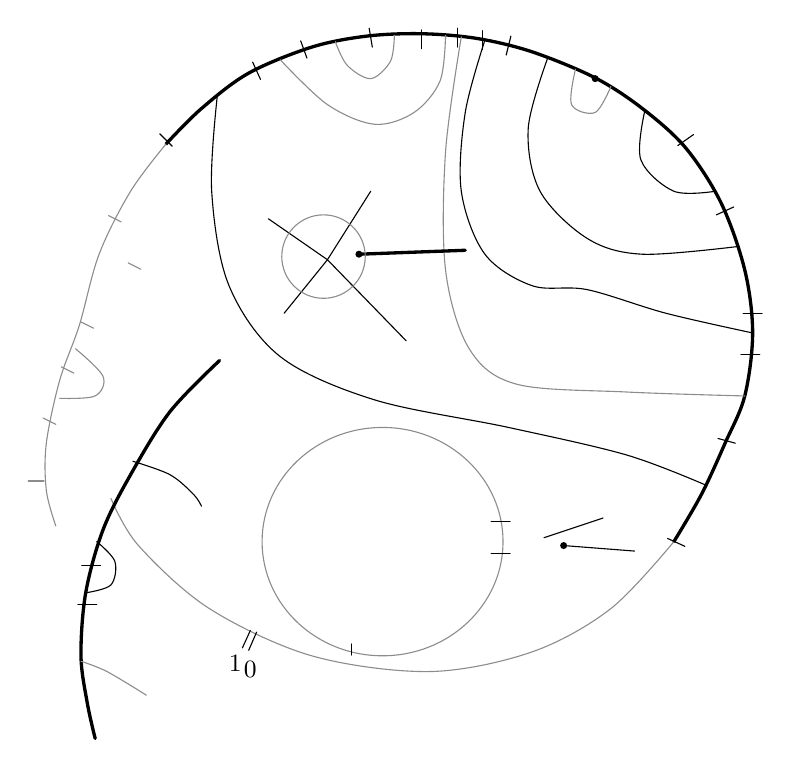
\begin{tikzpicture}[x=1mm,y=1mm,line cap=round,line join=round,font=\scriptsize]
\draw[very thick] plot[smooth, tension=0.55] coordinates {(21.5,-34) (26,-29.5) (32,-25) (40,-21.7) (47,-20.3) (54,-20) (61,-20.6) (68,-22.3) (76,-25.6) (82,-29.5) (87.5,-34.5) (92,-41.5) (95,-50) (96,-58) (95,-66) (92.5,-72) (89.5,-78.5) (86,-84.5)};
\draw[pencil] plot[smooth, tension=0.55] coordinates {(21.5,-34) (17,-40) (13,-48) (10.5,-57) (8,-64) (6.3,-72) (6.3,-78) (7.5,-82.5)};
\draw[pencil] plot[smooth, tension=0.55] coordinates {(86,-84.5) (78,-93) (68,-98.5) (55,-101) (40,-99) (27,-93) (18,-85) (14.5,-79)};
\draw (20.7,-32.7) -- (22.3,-34.3);
\draw (32.5,-23.6) -- (33.5,-25.8);
\draw (38.6,-20.9) -- (39.4,-23.1);
\draw (47.3,-19.3) -- (47.7,-21.7);
\draw (54,-19.5) -- (54,-21.9);
\draw (58.5,-19.3) -- (58.5,-21.7);
\draw (61.7,-19.6) -- (61.7,-22);
\draw (65.3,-20.3) -- (64.7,-22.7);
\draw (86.5,-34.2) -- (88.5,-32.8);
\draw (91.4,-43) -- (93.6,-42);
\draw (94.8,-55.5) -- (97.2,-55.5);
\draw (94.5,-60.7) -- (96.9,-60.7);
\draw (91.6,-71.4) -- (93.8,-72);
\draw (85.2,-84.1) -- (87.4,-85.1);
\node[pt] at (76,-25.7) {};
\draw[pencil] plot[smooth, tension=0.55] coordinates {(43,-21) (44.5,-24) (47.5,-25.7) (50,-23.5) (50.5,-20.2)};
\draw[pencil] plot[smooth, tension=0.55] coordinates {(36,-23.3) (42,-29) (48,-31.5) (53,-30) (56.3,-26) (57,-20.2)};
\draw plot[smooth, tension=0.55] coordinates {(28,-28) (27.3,-40) (29.5,-52) (36,-61) (48,-66.5) (65,-70) (80,-73.5) (90,-77.3)};
\draw[pencil] plot[smooth, tension=0.55] coordinates {(59,-20.4) (57,-35) (57,-50) (60,-60) (66,-64.5) (80,-65.5) (95,-66)};
\draw plot[smooth, tension=0.55] coordinates {(62,-20.8) (59.5,-30) (59,-40) (62,-48) (68,-52) (75,-52.5) (85,-55.5) (96,-58)};
\draw plot[smooth, tension=0.55] coordinates {(70,-23) (67.5,-32) (69,-40) (75,-46) (82,-48) (94.3,-47)};
\draw plot[smooth, tension=0.55] coordinates {(82.3,-29.8) (81.8,-36) (86,-40) (91.3,-40)};
\draw[pencil] plot[smooth, tension=0.55] coordinates {(73.5,-24.5) (73,-29) (76,-30) (78,-26.7)};
\node[pt] at (46,-48) {};
\draw[very thick] (46,-48) -- (59.5,-47.5);
\draw (34.5,-43.5) -- (42,-48.7) -- (52,-59);
\draw (47.5,-40) -- (42,-48.7) -- (36.5,-55.5);
\draw[pencil] (41.5,-48.3) circle[radius=5.3];
\node[pt] at (72,-85) {};
\draw (72,-85) -- (81,-85.7);
\draw (69.5,-84) -- (77,-81.5);
\draw[pencil] (49,-84.5) ellipse[x radius=15.3, y radius=14.5];
\draw (62.8,-82) -- (65.2,-82);
\draw (62.8,-86) -- (65.2,-86);
\draw (45,-97.5) -- (45,-98.9);
\draw[very thick] plot[smooth, tension=0.55] coordinates {(28.3,-61.5) (22,-68) (17,-76) (13.5,-83) (11.3,-91) (10.7,-99) (11.5,-105) (12.5,-109.5)};
\draw plot[smooth, tension=0.55] coordinates {(17.3,-74.3) (22,-76) (25,-78.5) (26,-80)};
\draw plot[smooth, tension=0.55] coordinates {(12.7,-84.5) (15,-87) (14.5,-90) (11.3,-91)};
\draw (10.8,-87.5) -- (13.2,-87.5);
\draw (10.3,-92.5) -- (12.7,-92.5);
\draw[pencil] plot[smooth, tension=0.55] coordinates {(10,-60) (13.5,-63.5) (12.5,-66) (8,-66.3)};
\draw[pencil] (14.2,-43.1) -- (15.8,-43.9);
\draw[pencil] (16.7,-49.1) -- (18.3,-49.9);
\draw[pencil] (10.7,-56.6) -- (12.3,-57.4);
\draw[pencil] (8.2,-62.3) -- (9.8,-63.1);
\draw[pencil] (5.9,-68.8) -- (7.5,-69.6);
\draw[pencil] (4,-76.8) -- (6,-76.8);
\draw[pencil] plot[smooth, tension=0.55] coordinates {(10.7,-99.7) (14,-101) (19,-104)};
\draw (31.2,-98) -- (32.2,-95.8);
\draw (32,-98.3) -- (33,-96);
\node[inner sep=1pt] at (30.3,-100) {\small $1$};
\node[inner sep=1pt] at (32.2,-100.7) {\small $0$};
\end{tikzpicture}
\end{document}
